\documentclass[12pt]{article}

\usepackage[utf8]{inputenc}
\usepackage{geometry}
\usepackage{amsmath, amssymb}
\usepackage{graphicx}
\usepackage{hyperref}
\usepackage{verbatim}
\usepackage{float}

\geometry{a4paper, margin=1in}

\usepackage{fancyhdr}
\pagestyle{fancy}
\fancyhead[L]{\textbf{University of Trento}}
\fancyhead[R]{MSc in Artificial Intelligence Systems}
\fancyfoot[C]{\thepage}

\title{\textbf{Autonomous Software Agents Project Report}}
\author{Bonetto Stefano (247179), Roman Simone (247181)}
\date{\today}

\begin{document}

\maketitle

\begin{abstract}
    This project develops an autonomous software agent designed to play a game, aiming to maximize points by collecting and delivering parcels. Utilizing a Belief-Desire-Intention (BDI) architecture, the agent senses the environment, manages beliefs, activates goals, selects plans, and executes actions to achieve its objectives. Initially focusing on a single agent's capabilities, including automated planning and belief revision, the project later extends to include a second agent, enabling communication and cooperative strategies. The system's performance is validated through simulation runs at d, demonstrating its efficiency in task completion through advanced AI techniques and multi-agent collaboration.
\end{abstract}

\section{Introduction}

The main goal of this project is to create an autonomous software agent that can play a game for the user. The game involves earning points by collecting and delivering parcels to a specific zone (the so called "\textit{delivery tiles}"). To do this, we're using a Belief-Desire-Intention (BDI) architecture. This architecture helps the agent understand its environment, decide on its goals, choose the best plans from a set of predefined options, and execute actions. It also allows the agent to continually update and adjust its plans to meet its objectives.

The project is split into two key parts. The first part focuses on building a single autonomous agent. This agent is designed to understand and manage information from its surroundings, adjust its beliefs, set goals, form intentions, and take actions. The agent has automated planning capabilities, meaning it can generate action plans when it identifies a new goal. We evaluate and validate the agent's performance by conducting a series of simulations across various levels, each with unique characteristics and challenges.

In the second part, we expand the project to include a second autonomous agent, enabling communication and cooperation between the two. This addition allows the agents to share information about their environment, exchange their goals, and coordinate their actions. In particular, we opt for a \texttt{MASTER-SLAVE} implementation where the \texttt{MASTER} is responsible for both the \texttt{best\_action} choiche of the himself and of the \texttt{SLAVE}. Again, we test and validate the performance of this multi-agent system through simulations.

By using advanced strategies and cooperative dynamics between multiple agents, this project aims to create a smart, efficient system that can effectively complete the game's objectives. Through the development and testing stages, the system shows its capability to maximize performance by managing tasks and coordinating actions between the agents.

\section{Belief}

The beliefs of our agent essentially form its understanding of the environment in which it operates. These beliefs are shaped by the agent's perceptions and are constantly updated as it encounters new stimuli. This ongoing process ensures that the agent's view of the world remains current and responsive to changes, allowing it to make informed decisions as it navigates its tasks.

The key perceptions that our agent is capable of detecting include:

\begin{itemize}
    \item Map perception
    \item Parcels' perception
    \item Agents' perception
\end{itemize}

Based on Deliveroo's current level's parameters, our agent has a field of view that is determined by the furthest tile it can see.

\subsection{Map sensing}

At the start of each game, the map is perceived by the agent. The tiles on the map can be of four different types:

\begin{itemize}
    \item Blocked tiles (empty or not\_tile)
    \item Walkable spawning tiles (where parcels can spawn)
    \item Walkable non-spawning tiles
    \item Delivery tiles
\end{itemize}

The server sends each agent a JSON file containing an entry for each non-empty tile in the following format:

\begin{center}
    \texttt{\{ x: 0, y: 0, delivery: true, parcelSpawner: false \}}
\end{center}

This JSON file is used to create a matrix that represents the map more effectively, with the following values for each type of tile:

\begin{table}[h]
    \centering
    \begin{tabular}{|c|c|}
        \hline
        \textbf{0} & Blocked tiles \\
        \hline
        \textbf{1} & Walkable non-spawning tiles \\
        \hline
        \textbf{2} & Delivery tiles \\
        \hline
        \textbf{3} & Walkable spawning tiles \\
        \hline
    \end{tabular}
    \label{tab}
\end{table}

To store the data we create a class \texttt{Map}.

\subsubsection{MyMap}
This instantiation of the \texttt{Map} class helps us to retain all the data related to the map, including:

\begin{itemize}
    \item \texttt{original\_map}: the initial map sent by the server.
    \item \texttt{map}: the map used by the agent to plan its behavior, which includes some extra values for agents sensed (see section \ref{agents} for more details).
    \item \texttt{deliveryCoordinates}: the coordinates of each delivery tile.
    \item \texttt{spawningCoordinates}: the coordinates of each spawning tile.
    \item \texttt{width} and \texttt{height}: the dimensions of the map.
    \item \texttt{parcel\_reward\_avg}, \texttt{parcel\_observation\_distance} and \texttt{decade\_frequency} : some configuration parameters depending on the level we're playing, including the average reward of the parcels, the maximum distance from which we can sense a parcel and the decade frequency (see better at paragraph \ref{config_params}) .
    \item \texttt{myBeliefset}: updated based on the current state of the map (with \texttt{updateBeliefset()} method), it stores information about the existence and relationships of tiles. This is used for the formulation of the PDDL problem.
\end{itemize}

Finally the \texttt{updateMap(x, y, value)} method is used to update the value of a given tile when an agent is sensed (see section \ref{agents} for more details).

\subsection{Parcels' sensing}

Parcels perception is linked with the \texttt{parcel\_observation\_distance} level parameter, which indicates the maximum distance within which the agent can detect parcels. 

Whenever a parcel enters in the field of view of the agent, the agent received from the server informations about the parcel, including his \texttt{id}, his \texttt{coordinates} and the \texttt{reward}.    

\subsubsection{MyData and CollaboratorData}

\texttt{MyData} and \texttt{CollaboratorData} are instances of the \texttt{AgentData} class. We use \texttt{MyData} to store the data of the current agent instance. If the current instance is a \texttt{MASTER} agent, in addiction we store the data received from the \texttt{SLAVE} in \texttt{CollaboratorData}.

Each instance of \texttt{AgentData} is composed of the following elements:

\begin{itemize}
    \item \texttt{name}: name of the agent
    \item \texttt{id}: id of the agent
    \item \texttt{pos}: position of the agent, updated with the onYou promise
    \item \texttt{role}: role may be \texttt{SLAVE} (the one who receive the handshake and ACK it back) or \texttt{MASTER} (the one who send the handshake). 
    \item \texttt{parcels}: list of parcels sensed using onParcelSensing
    \item \texttt{inmind}: total score of parcels collected by the agent
    \item \texttt{options}: this list store the list of option that are formulated (all of them).
    \item \texttt{best\_option}: this is simply the best option of the previous list (w.r.t. the utility).
    \item \texttt{adversaryAgents}: list of agents updated according to agent perceiving. 
    \item \texttt{parcelsInMind}: list of parcels store in the head of the agent (already picked up).
\end{itemize}

\subsection{Agents' sensing}
\label{agents}
We aim to simplify the handling of agents' sensing: when an agent is detected, three operations are performed:

\begin{enumerate}
    \item The new sensed agent is added to \texttt{MyData.adversaryAgent} list;
    \item We want to treat the tile where the agent is located as an empty tile, so we update the map using \texttt{updateMap} method of \texttt{MyMap};
    \item Finally we update the PDDL belief-set formulation to ensure that the tile where the agent has been sensed won't be considered as part of the usable path for the given intention.
\end{enumerate}

The second step is based on the \texttt{original\_map} sensed at the beginning of the game. When an agent is detected, the current \texttt{map} is updated by starting with a deep copy of the \texttt{original\_map} and setting the tile where the agent is detected to $-1$. 

Then, during the initialization of our PDDL problem, only tiles with values greater than $0$ will be considered (walkable tiles), so tiles with values of $0$ (empty tiles) or $-1$ ("agents" tiles) will be ignored in the PDDL problem formulation.

\subsubsection{Handling Agent Collisions}

Unfortunately, this isn't sufficient to completely avoid collisions between agents, as they are likely moving.

However, we've tried various techniques to prevent or manage collisions between both cooperative and adversarial agents. The main issue with our implementation is that once the PDDL plan is computed and the corresponding path is returned, the agent begins moving, and we're unable to check for potential collisions with other agents at each step.  

First, we decided to try a very invasive technique: for each path computed for the \texttt{SLAVE}, we reset the map and then set the entire path as unused tiles (assigned a value of $-2$) on the \texttt{MASTER} side, effectively removing these tiles from the \texttt{MASTER}'s path calculation. 

\begin{figure}[H]
    \centering
    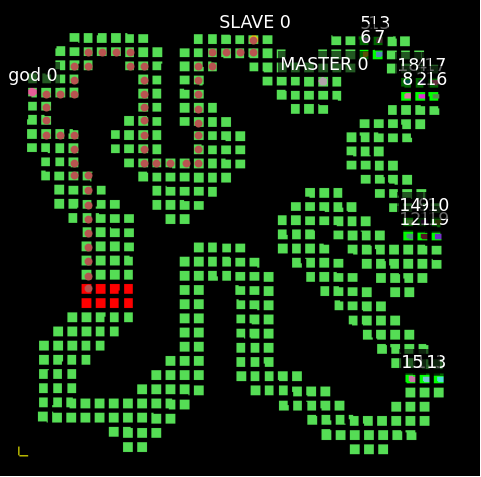
\includegraphics[width=0.5\linewidth]{path_-1.png}
    \caption{\centering \textit{Scenario example}}
    \label{fig:enter-label}
\end{figure}

As we can see from the upper figure, the \texttt{SLAVE} intends to put down parcels and begins following the red path, forcing the \texttt{MASTER} to take a longer route around the map. This results in a highly suboptimal solution, significantly reducing the overall score.

However, this technique is both drastic and suboptimal. If the \texttt{SLAVE} completely blocks the \texttt{MASTER}'s path, or, as shown in the figure, blocks the optimal path to the \texttt{MASTER}'s goal, it can lead to inefficient or even unfeasible solutions. This approach could prevent the \texttt{MASTER} from finding an effective route, significantly hindering overall performance.


\section{Configuration Problem Parameters}

\label{config_params}

Whenever a new game begins, you can select a level from those available on the server. Each level comes with specific fixed parameters that we utilize to optimize our agent's performance. These parameters are extracted using the following callback, which is triggered once at the start of the game:

\begin{verbatim}
    client.onConfig((config) => {
    let movement_duration = config.MOVEMENT_DURATION;
    // ...others assignations...
    });
\end{verbatim}

First of all we want to compute the so called \texttt{decade\_frequency} which will be useful when computing utility for the parcels: 

\begin{equation}
    decade\_frequency = \frac{agent\_movement\_duration}{parcel\_decading\_inteval}
\end{equation}

This ratio quantifies the rate at which a parcel's score diminishes with each step the agent takes, helping to align the measurement units between the agent and the parcel.

In certain levels, the \texttt{parcel\_decaying\_interval} is set to \texttt{"infinite"}; in such cases, we assign it a value of \texttt{Number.MAX\_VALUE}.

Then, our focus is on \texttt{parcel\_observation\_distance}, which we will use to calculate the spawning score of a single tile. This allows us to identify the optimal tile to serve as the goal for a random move, aiming to maximize the number of spawning tiles within a \texttt{POD} $\times$ \texttt{POD} window.

Lastly, we extract the \texttt{parcel\_reward\_avg} that we'll use to determine a threshold for the \texttt{go\_put\_down} intention. This threshold is specified at paragraph \ref{variant_go_put_down}.

\section{Agent Loop}

\subsection{Utility functions and intention selection}

\subsubsection{Put-down utility}

For the \texttt{go\_put\_down} intention, we use the following utility function to determine the best course of action for the agent:

\begin{equation}
    \text{utility} = \text{scoreInMind} - decade\_frequency \times \text{dist}(\text{me}, \text{nearestDelivery}) \times \text{nParcelsInMind}
\end{equation}

Here, $\text{scoreInMind}$ represents the total reward the agent has collected from the parcels it is currently carrying. 


Consequently, at each timestep, the total $\text{scoreInMind}$ decreases by one unit for each parcel the agent is carrying. The utility function, therefore, takes into account both the reward the agent is holding and the decay of this reward over time due to the distance to the nearest delivery zone and the number of parcels.

\subsubsection{Variant when \texttt{parcel\_decading\_interval} == "infinite"}

\label{variant_go_put_down}

When \texttt{PARCEL\_DECAYING\_INTERVAL} is set to infinite (depending on the map we're playing), it's advantageous to wait and collect as many parcels as possible before occasionally putting them down once we achieve a high \texttt{inMindScore}. To implement this strategy, we add a condition based on the average score of the spawned parcels multiplied by a constant (e.g., fixed at 10):

\begin{verbatim}
        if (inmind_score > parcel_avg_reward * MULT_THRESH_GO_PUT_DOWN) {
            // GO_PUT_DOWN set as best_option
        }
\end{verbatim}

\subsubsection{Pick-up utility}

The utility function for the \texttt{go\_pick\_up} intention is more complex and involves several components:

\begin{equation}
    \text{utility} = \text{RewardParcel} + \text{RewardInMind} - f \times \text{dist}(\text{me}, \text{delivery}) \times (\text{numParcelInMind} + 1)
\end{equation}

In this equation, $\text{RewardInMind}$ is calculated as:

\begin{equation}
    \text{RewardInMind} = \text{scoreInMind} - f \times \text{dist}(\text{me}, \text{parcel}) \times \text{numParcelInMind}
\end{equation}

This term accounts for the current reward the agent is holding, adjusted for the decay due to the distance to the parcel and the number of parcels in mind.

Similarly, $\text{RewardParcel}$ is defined as:

\begin{equation}
    \text{RewardParcel} = \text{scoreParcel} - f \times \text{dist}(\text{me}, \text{parcel})
\end{equation}

This term represents the reward of the parcel the agent is considering picking up, minus the decay caused by the distance to this parcel.

Furthermore, we introduce a penalty to the utility function if the distance between the agent and a parcel is greater than the distance between the nearest agent and the same parcel. This penalty is included as follows:

\begin{equation}
    \text{utility} = \text{utility} - \text{malus} \times (\text{dist}(\text{me}, \text{parcel}) - \text{dist}(\text{nearestAgent}, \text{parcel}))
\end{equation}

The term $\text{malus}$ represents the penalty factor, which is applied to the difference between the agent's distance to the parcel and the nearest agent's distance to the same parcel. This ensures that the agent considers the proximity of other agents when deciding whether to pick up a parcel, thus optimizing task distribution among multiple agents.

\subsection{Intention revision}

\section{Planning}

One of the most crucial aspects of our agent's functionality is the action planning process, which involves determining the optimal path to reach a given goal. 

To assess the distances between tiles, we use the Manhattan distance metric. Initially, we've implemented a basic planner that relies on Breadth-First Search (BFS) to explore and identify the most efficient path.

\subsection{Initial version - BFS}

\textbf{Breadth-First Search (BFS)} is an algorithm used to explore graphs or grids. It starts at the initial tile and explores all its neighbors before moving to the next level. By expanding outward tile by tile, BFS guarantees finding the shortest path in unweighted grids, making it ideal for scenarios like pathfinding where uniform movement cost is assumed.

\subsection{PDDL}

A \textbf{PDDL-based planner} takes this description and generates a plan, which is a sequence of actions that transforms the initial state into the desired goal state. 

The planner systematically explores possible actions, considering their preconditions and effects, to build a feasible plan that accomplishes the objectives laid out in the PDDL.

In our implementation, we set a fixed domain for our PDDL problems that specifies the allowed predicates and their implementations allowed and their respective parameters, preconditions and effects:

\begin{verbatim}
    (:action move-down
        :parameters (?tile1 ?tile2)
        :precondition (and (at ?tile1) (down ?tile2 ?tile1))
        :effect (and (at ?tile2) (not (at ?tile1)))
    )
\end{verbatim}

To select the most optimal choice for performance, we estimate the utility of each option by evaluating the path provided by the BFS formulation rather than using the PDDL approach. Once the optimal option, termed \texttt{best\_option}, is identified, we then formulate the corresponding PDDL problem for execution:

\begin{verbatim}
    ;; problem file: name_of_problem_file.pddl
    (define (problem default)
    (:domain default)
    (:objects ... )
    (:init ... )
    (:goal ... ) 
\end{verbatim}

where:

\begin{itemize}
    \item \texttt{domain} refers to the file we have previously defined;
    \item  \texttt{objects} is the list of all the instances on the environment that can interact (parcels, tiles, etc...);
    \item \texttt{init} explicate the initial scenario of the environment (e.g. the list of tiles with the list of action we can perform starting from those tiles, the initial position of the agent, etc...);
    \item \texttt{goal} is the final effect we want to obtain 
\end{itemize}

To compute the PDDL plan, we can choose between running it locally or using an online service. We opt to perform it locally, as this is the faster option. Additionally, we leverage tools like those available at \href{https://github.com/AI-Planning/planning-as-a-service}{AI-Planning's planning-as-a-service} repository to facilitate the process.
 

\subsection{Random move}

When determining the random move to perform when no parcel is sensed, we explored various approaches and strategies. 

Ultimately, we developed the function \texttt{find\_random\_deliveryFarFromOther}, which is split into two cases:

\begin{itemize}
\item If the current agent's role is \texttt{SLAVE} (in a multi-agent scenario) or \texttt{NOTHING} (in a single-agent scenario), the agent goal is to reach the best scoring tile according to \texttt{getBestSpawningCoordinates} (see after the implementation), if the agent has tried yet to randomly move to the best tile, he reach the nearest delivery tile, hoping that something appears in the meantime.
\item Otherwise, if the current agent's role is \texttt{MASTER}, the random move takes into account the goal of the collaborator agent (the coordinates he wants to reach by doing the \texttt{best\_option}). In this case, the \texttt{MASTER} agent aims to reach the furthest spawning tile to the \texttt{SLAVE}'s position. If it's yet in the furthest spawning tile , he simply reach the second furthest tile from the collaborator's goal coordinates.
\end{itemize}

In both cases, an option with the predicate \texttt{go\_random\_delivery} is added to the options' queue with a very low utility. This ensures that it will be selected as the best option only if no other more favorable options are available in the queue (in practice, this option is selected only when it is not particularly beneficial to pick up parcels in the environment or if there are no parcels present. This mechanism ensures that the agent prioritizes more advantageous actions before resorting to random movement).

\section{Communication}
A fundamental aspect of the multi-agent scenario is the communication between the agents.

The core concept behind our implementation of the collaboration method is the creation of a shared belief set, comprising all parcels observed by both agents along with their respective utility values.

We are particularly focused on managing parcels seen by both agents. In such cases, we compare the utility values from each agent's perspective and assign the task of picking up the parcel to the agent for whom it is more advantageous.

Notice that all this computation is done \texttt{MASTER}-side while the \texttt{SLAVE} only sends his state (\texttt{MyData} see better on paragraph \ref{belief}) and receive back his state updated with the actual \texttt{options} and especially the \texttt{best\_option}. 

\subsection{Handshake}

To establish communication in our multi-agent system, we implemented a handshake process to synchronize and identify the roles of the agents. This process begins with a short delay to ensure synchronization. The first agent that established connection with the server then sends a broadcast message containing its identity and a tag indicating the start of the handshake.

The receiving agent listens for this message and, upon verification, assumes the role of \texttt{SLAVE}, sending an acknowledgment back. The initiating agent, upon receiving the acknowledgment, identifies itself as the \texttt{MASTER}. This exchange finalizes the handshake, ensuring both agents know each other's roles and are ready to collaborate effectively. 

\subsection{Belief sharing}
\label{belief}

As previously mentioned, the process of determining the best options for both the \texttt{SLAVE} and the \texttt{MASTER} agents is centralized and conducted on the \texttt{MASTER} side. This approach ensures that both agents operate under a coherent strategy.

The \texttt{SLAVE} agent's role in this process is to transmit its current state information to the \texttt{MASTER}. This state includes relevant data such as its position, observed parcels, and other information that could influence decision-making. Once this data is sent, the \texttt{SLAVE} awaits update.

Upon receiving the \texttt{SLAVE}'s state, the \texttt{MASTER} processes the information, considering both its own state and the data received from the \texttt{SLAVE}. The \texttt{MASTER} then computes a comprehensive set of options for both agents. Among these options, the \texttt{MASTER} identifies the optimal choice, or best\_option, for both the \texttt{SLAVE} and itself.

The \texttt{MASTER} subsequently sends a response back to the \texttt{SLAVE}, which includes an updated version of the \texttt{CollaboratorData} structure (\texttt{SLAVE} data). This updated data set contains the newly computed options (for instance, the choices for picking up parcels that the \texttt{SLAVE} couldn't find on its own) along with the selected best option. The \texttt{SLAVE} then acts based on this guidance, ensuring coordinated action between the agents. This process facilitates effective collaboration, with the \texttt{MASTER} guiding the overall strategy while the \texttt{SLAVE} follows the directives to achieve the shared goals.

\begin{verbatim}
    await client.say(CollaboratorData.id, {
        hello: "[INFORM]",
        data: data,
        time: Date.now()
    });
\end{verbatim}

\begin{comment}
    \begin{thebibliography}{9}
\bibitem{esempio}
Autore, \textit{Titolo del libro}, Editore, Anno.

% Aggiungi altre voci bibliografiche qui
\end{thebibliography}

\end{comment}

\end{document}
